\documentclass[xcolor=dvipsnames]{beamer}
\mode<presentation>{}
\usetheme{Frankfurt}
\usecolortheme{dolphin}
\useinnertheme{circles}
\useoutertheme{split}
\usepackage{animate}
\usepackage{xcolor}
\usepackage{movie15}
\usepackage{media9}
\usepackage[framemethod=tikz]{mdframed}
\usepackage{etoolbox}
\title{Hackathon}
\author{Senthilkumar Sockalingam Kathiresan \& Yannick Weitz}
\setbeamercolor{section in toc}{fg=black}
\setbeamercolor{subsection in toc}{fg=ForestGreen}
\setbeamertemplate{subsection in toc}[subsections numbered]
\setbeamercolor{subsection number projected}{bg = black, fg = white}
\setbeamercolor{section number projected}{bg=black,fg=white}
\setbeamercolor{structure}{bg=black, fg = ForestGreen}

\setbeamertemplate{itemize items}[circle]
\setbeamercolor{itemize item}{fg=ForestGreen}
\setbeamertemplate{itemize subitem}{\color{black}$\blacktriangleright$}
\AtBeginSection[]{
\begin{frame}{Table of Contents}
\tableofcontents[ 
currentsection,currentsubsection, 
hideothersubsections, 
sectionstyle=show/hide,
currentsubsubsectionstyle=show/shaded,
]  
\end{frame}
}

\mdfdefinestyle{stop}{
  roundcorner=2pt,
  linewidth=5pt,
  linecolor=red!80,
  backgroundcolor=red!20
}
\mdfdefinestyle{start}{
  roundcorner=2pt,
  linewidth=5pt,
  linecolor=green!80,
  backgroundcolor=green!20
}
\mdfdefinestyle{normal}{
  roundcorner=2pt,
  linewidth=5pt,
  linecolor=gray!80,
  backgroundcolor=gray!20
}

\begin{document}

\begin{frame}
\titlepage
\end{frame}

\begin{frame}
\tableofcontents[section]
\end{frame}

\section{Introduction}


\begin{frame}{personal description}
\begin{columns}

\begin{column}[b]{0.5\textwidth}
\begin{center}
\textbf{Senthil :}

\begin{itemize}
\item hi
\end{itemize}

\end{center}
\end{column}
\begin{column}[b]{0.5\textwidth}  %%<--- here
\begin{center}
\textbf{Yannick :}

\begin{itemize}
\item Age: 22
\medskip
\item From: Germany
\medskip
\item Studied: Biomimetics
\end{itemize}

\end{center}
\end{column}
\end{columns}

\end{frame}
\section{ROS}

\begin{frame}{what have we learned}
\begin{itemize}
\item<1-> creating workspace
\item<2-> how nodes work
\item<3-> how topics work
\item<4-> how mesages work
\end{itemize}
\end{frame}

\section{Hackathon}

\subsection{First task}
\begin{frame}{First task}

\only<1,4>{\begin{mdframed}[style=normal]\begin{center}\huge Start \end{center}\end{mdframed}}
\only<2-3>{ \begin{mdframed}[style=start]\begin{center}\huge Start \end{center}\end{mdframed}}
\only<1-3> {\begin{mdframed}[style=normal]\begin{center}\huge Stop \end{center}\end{mdframed}}
\only<4>{ \begin{mdframed}[style=stop]\begin{center}\huge Stop \end{center}\end{mdframed}}
\begin{flushleft} \color<2>[rgb]{0.25,0.95,0.11} \huge Left  \hspace{7.7cm} \color<2>[rgb]{0,0,0}\color<3>[rgb]{0.25,0.95,0.11}\huge Right \end{flushleft}
\medskip
\only<1>{ \begin{center} 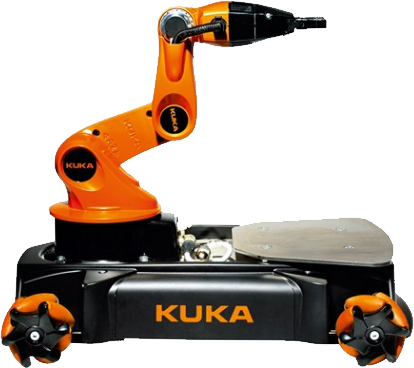
\includegraphics[scale=0.15]{youbot} \end{center}}
\only<2>{\begin{flushleft} \reflectbox{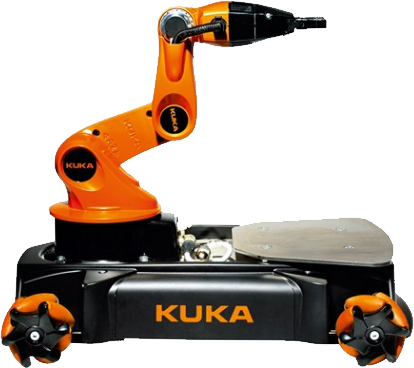
\includegraphics[scale=0.15]{youbot}} \end{flushleft} }
\only<3-4>{\begin{flushright} 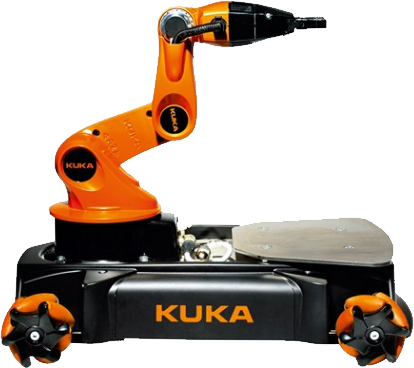
\includegraphics[scale=0.15]{youbot} \end{flushright} }
\end{frame}

\begin{frame}

\large Speed: \only<1,5,7>{0 $\frac{m}{s}$}\only<2-4>{1 $\frac{m}{s}$}\only<6>{3 $\frac{m}{s}$}
\begin{flushright}
\color<2-4,6>[rgb]{0.25,0.95,0.11}\huge Right
\end{flushright}

\begin{flushleft}
\only<1-2,6>{\Huge 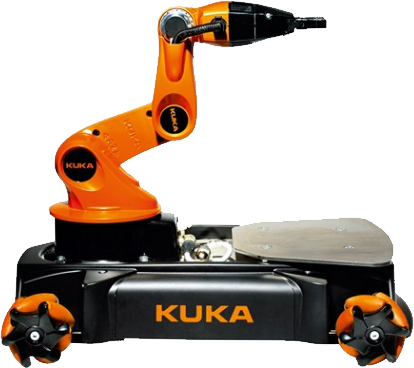
\includegraphics[scale=0.15]{youbot}}
\only<3>{\hspace{2.3cm}\Huge 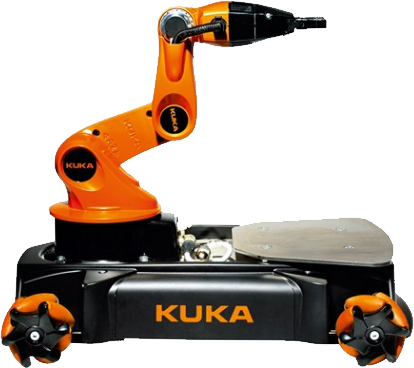
\includegraphics[scale=0.15]{youbot}}
\only<4>{\hspace{4.6cm}\Huge 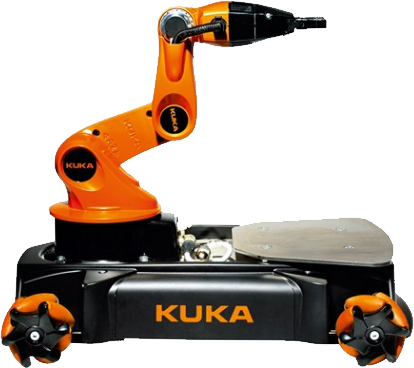
\includegraphics[scale=0.15]{youbot}}
\only<5,7>{\hspace{6.9cm}\Huge 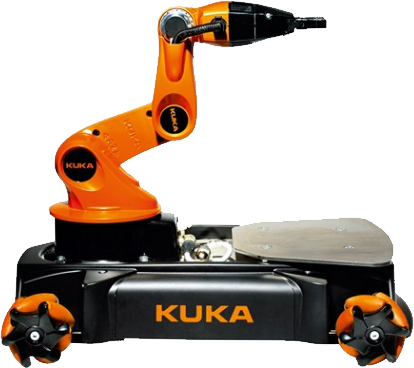
\includegraphics[scale=0.15]{youbot}}
\end{flushleft}

\begin{flushleft}
\hspace{0.5cm} \huge \color<2->[rgb]{0.25,0.95,0.11}{0m} \hspace{0.5cm}\vline \hspace{0.5cm} \color<2,6>[rgb]{0,0,0}1m \hspace{0.5cm}\vline \hspace{0.5cm} \color<3>[rgb]{0,0,0}2m \hspace{0.5cm}\vline \hspace{0.5cm} \color<4>[rgb]{0,0,0}3m \hspace{0.5cm} 
\end{flushleft}
\end{frame}

\subsubsection{Approach}

\begin{frame}



\end{frame}

\subsubsection{limitations}

\begin{frame}

\end{frame}

\subsection{Second task}
\begin{frame}

\end{frame}

\section{course}


\section*{end}

\begin{frame}
\begin{center}
\Huge Thank you for listening !
\end{center}
\end{frame}
\end{document}
